\documentclass[english,handout]{beamer}






 
%\usepackage{mathptmx}
%\renewcommand{\sfdefault}{lmss}
\usepackage[T1]{fontenc}
%\usepackage[latin9]{inputenc}
\usepackage[utf8]{inputenc}

\synctex=-1

\usefonttheme{professionalfonts}

%\setbeamertemplate{navigation symbols}{}
%\setbeamertemplate{caption}[numbered]


\useinnertheme{rectangles}
%http://tex.stackexchange.com/questions/11168/change-bullet-style-formatting-in-beamer

 \AtBeginDocument{
  \addtolength\abovedisplayskip{-0.4\baselineskip}%
  \addtolength\belowdisplayskip{-0.4\baselineskip}%
}%change the space between text lines and the math formula


\usepackage{pifont}
%Postscript ZipfDingbats font
%the command \ding{number}, will print the specified symbol

\usepackage{fontawesome}
%icon package
\DeclareFontFamily{U}{FontAwesomeOne}{}
\DeclareFontShape{U}{FontAwesomeOne}{m}{n}{<-> FontAwesome--fontawesomeone}{}
\DeclareRobustCommand\FAone{\fontencoding{U}\fontfamily{FontAwesomeOne}\fontseries{m}\fontshape{n}\selectfont}
\DeclareFontFamily{U}{FontAwesomeTwo}{}
\DeclareFontShape{U}{FontAwesomeTwo}{m}{n}{<-> FontAwesome--fontawesometwo}{}
\DeclareRobustCommand\FAtwo{\fontencoding{U}\fontfamily{FontAwesomeTwo}\fontseries{m}\fontshape{n}\selectfont}
\DeclareFontFamily{U}{FontAwesomeThree}{}
\DeclareFontShape{U}{FontAwesomeThree}{m}{n}{<-> FontAwesome--fontawesomethree}{}
\DeclareRobustCommand\FAthree{\fontencoding{U}\fontfamily{FontAwesomeThree}\fontseries{m}\fontshape{n}\selectfont}

%ftp://ftp.dante.de/tex-archive/fonts/fontawesome/doc/fontawesome.pdf
%http://tug.ctan.org/info/symbols/comprehensive/symbols-a4.pdf


\usepackage{amsmath,amssymb,amsfonts,bm,mathrsfs,mathtools}

\usepackage{tikzsymbols}
%\usepackage[tikz]{bclogo}



\usepackage{perpage}
\MakePerPage{footnote} %reset for each page
%\renewcommand{\thefootnote}{\fnsymbol{footnote}} %use symbol, limit less than 9 symbols



%%%% HIGHTLIGHT  and annotation &=%%%%%%%%
\usepackage{color,xcolor}
 \usepackage{todonotes}

\usepackage[normalem]{ulem}

\usepackage[many]{tcolorbox}

\tcbset{fonttitle=\scriptsize}
\tcbset{highlight math style={enhanced,
  colframe=red!40!black,colback=yellow!20!white,arc=2pt,boxrule=.2pt,
  }}
  \newtcbox{\otherbox}[1][]{nobeforeafter,math upper,tcbox raise base,
enhanced,frame hidden,boxrule=0pt,interior style={top color=green!10!white,
bottom color=green!10!white,middle color=green!50!yellow},
fuzzy halo=1pt with green,#1}
%%\tcbhighmath{math here}
%% \otherbox{math here}



%%%%% HIGHLIGHT %%%%%%
\newcommand{\hb}[1]{{\color{blue}{#1}}}
%\noindent\rule{\textwidth}{.5pt}

%:
\usepackage{soul}

\newcommand\hcancel[2][black]{\setbox0=\hbox{$#2$}%
\rlap{\raisebox{.45\ht0}{\textcolor{#1}{\rule{\wd0}{1pt}}}}#2}
%cross to delete

\newcommand{\mcb}[2]{\colorbox{#1}{$\displaystyle #2$}}
%highlight math

\newcommand{\hlfancy}[2]{\sethlcolor{#1}\hl{#2}}
%specified color , for\hl

\newcommand\myhl{\bgroup\markoverwith
  {\textcolor{yellow}{\rule[-.5ex]{2pt}{2.5ex}}}\ULon}



\mode<presentation>{ \usetheme{boxes} }

%write Matlab code
\usepackage{listings}
 \definecolor{dkgreen}{rgb}{0,0.6,0}
\definecolor{gray}{rgb}{0.5,0.5,0.5}
\definecolor{mauve}{rgb}{0.58,0,0.82}
\lstset{frame=tb,
  language=Matlab,
  aboveskip=3mm,
  belowskip=3mm,
  showstringspaces=false,
  columns=flexible,
  basicstyle={\small\ttfamily},
  numbers=none,
  numberstyle=\tiny\color{gray},
  keywordstyle=\color{blue},
  commentstyle=\color{dkgreen},
  stringstyle=\color{mauve},
  breaklines=true,
  breakatwhitespace=true
  tabsize=3
}

\usepackage[lastexercise]{exercise}

\newtheorem{ex}{Exercise}
\newtheorem{property}{Property}
\newtheorem{ag}{Algorithm}
\newtheorem{remark}{Remark}
\newtheorem{den}{definition}
\newtheorem{assumption}{Assumption}


\usepackage[nosolutionfiles]{answers}
\Newassociation{sol}{Solution}{ans}



\usepackage{empheq}
\usepackage{comment}
%\usepackage{lscape}
\usepackage{multirow}
\usepackage{url,hyperref}

\hypersetup{
 %   bookmarks=true,         % show bookmarks bar?
    unicode=false,          % non-Latin characters in Acrobat's bookmarks
    pdftoolbar=true,        % show Acrobat's toolbar?
    pdfmenubar=true,        % show Acrobat's menu?
    pdffitwindow=false,     % window fit to page when opened
    pdfstartview={FitH},    % fits the width of the page to the window
    pdftitle={My title},    % title
    pdfauthor={Author},     % author
    pdfsubject={Subject},   % subject of the document
    pdfcreator={Creator},   % creator of the document
    pdfproducer={Producer}, % producer of the document
    pdfkeywords={keyword1} {key2} {key3}, % list of keywords
    pdfnewwindow=true,      % links in new window
    colorlinks=true,       % false: boxed links; true: colored links
    linkcolor=red,          % color of internal links (change box color with linkbordercolor)
    citecolor=green,        % color of links to bibliography
    filecolor=magenta,      % color of file links
    urlcolor=cyan           % color of external links
}


\usepackage{subfigure,epsfig,graphicx,graphics}

\DeclareGraphicsRule{.tif}{png}{.png}{`convert #1 `dirname #1`/`basename #1 .tif`.png}
   \DeclareGraphicsExtensions{.pdf}




\newcommand{\hw}{ {\underline{\tt Homework }} }
\newcommand{\hws}{ {\underline{\tt Homework$\star$}} }
\newcommand{\optional}{ {\it optional} }

\newcommand{\MATLAB}{ \texttt{MATLAB}}
\newcommand{\python}{ \texttt{python}}
\newcommand{\Rlang}{ \texttt{R}}
\newcommand{\SAS}{ \texttt{SAS}}
\newcommand{\MC}{Markov Chain}


\newcommand{\tm}{transition matrix}
\newcommand{\rv}{random variable}
\newcommand{\spl} {supervised learning }
 

\newcommand{\dis}{\underline{\tt discussion}: }
\newcommand{\pri}{\underline{\tt principle}: }




\newcommand{\bq}{\scalebox{6}{\textbf{?} }}
\newcommand{\sq}{\scalebox{2}{\textbf{?} }}
\newcommand{\ck} {  {\scalebox{0.8} {\Interval}   } }

\newcommand{\eps}{\varepsilon}
\newcommand{\To}{\longrightarrow}

% 
\newcommand{\Dcal}{\mathtt{D}}
\newcommand{\Hcal}{\mathcal{H}}
\newcommand{\Ecal}{\mathcal{E}}
\newcommand{\Xcal}{\mathcal{X}}
\newcommand{\Ycal}{\mathcal{Y}}
\newcommand{\Zcal}{\mathcal{Z}}

%%Calculus 

\renewcommand{\d}{\ensuremath{\mathrm{d}}}
\newcommand{\dt}{ \ensuremath{\mathrm{d} t } }
\newcommand{\dx}{ \ensuremath{\mathrm{d} x} }
\newcommand{\dy}{ \ensuremath{\mathrm{d} y } }

%indicator function
\newcommand{\indf}{ \ensuremath{\mathbf{1} } }



%probability
\newcommand{\p}{ \mathbb{P}}
\newcommand{\prob}{{\Pr}}
\newcommand{\PP}{\mbox{PP}}%Poisson process
%condition prob
\newcommand{\cPr}[2]{{\Pr\left(#1\mid #2\right)}}

\newcommand{\FF}{{\mathbb{F}}}

\newcommand{\e}{ \operatorname{\mathbb E}}
\newcommand{\Var}{\operatorname{\mathbb{V} }}
\newcommand{\var}{\operatorname{\text{Var} }}
\newcommand{\MSE}{\operatorname{\text{MSE} }}

\newcommand{\Std}{\operatorname{std}}
\newcommand{\Cov}{\operatorname{cov}}

%Matrix  %mathbf
\newcommand{\Pb}{{\mathbf{P}}}
\newcommand{\Qb}{{\mathbf{Q}}}
\newcommand{\Mb}{{\mathbf{M}}}
\newcommand{\cb}{\mathbf{c}}
\newcommand{\bb}{{\mathbf{b}}}

\newcommand{\Tb}{\mathbf{T}}

\newcommand{\Wb}{\mathbf{W}}
\newcommand{\wb}{\mathbf{w}}
\newcommand{\Xb}{\mathbf{X}}

\newcommand{\xb}{\mathbf{x}}

\newcommand{\Wtn}{\mathbb{W}}
\newcommand{\btn}{\mathbf{b}}



\newcommand{\eye}{{\mathbf{I}}}
%identity matrix
\newcommand{\onem}{{\mathbb{1}}}
\newcommand{\idor}{\mathbf{1}}
\newcommand{\ii}{\mathbf{i}}
%imaginary symbol

\usepackage{tikz}

%State number
\newcommand{\snum}[1]{ \raisebox{.5pt}{\textcircled{\raisebox{-.9pt} {#1}}}}

 \usetikzlibrary{arrows}
\usetikzlibrary{shapes}

%\newcommand{\snum}[1]{%
 % \tikz[baseline=(char.base)]\node[anchor=south west, draw,rectangle, rounded corners, inner sep=1.4pt, minimum size=5mm,
   % text height=1.3mm](char){\ensuremath{#1}} ;}

\newcommand*\circled[1]{\tikz[baseline=(char.base)]{
            \node[shape=circle,draw,inner sep=.4pt] (char) {#1};}}


%real number
\newcommand{\Real}{{\mathbb{R}}}
%integer
\newcommand{\ZZ}{\mathbb{Z}}
%positive integer
\newcommand{\NN}{\mathbb{N}}



\newcommand{\inpd}[2]{\left\langle #1, #2 \right\rangle}
\newcommand{\abs}[1]{\left\vert#1\right\vert}
\newcommand{\norm}[1]{\left\|#1\right\|}
\newcommand{\wt}[1]{{\widetilde{#1}}}
\newcommand{\set}[1]{\left\{#1\right\}}
\newcommand{\partiald}[2]{  \frac{\partial #1 }{\partial #2}}



\newcommand{\ie}{{\it{i.e.}}}



\newcommand{\transpose}{\textsf{T}} % or, \intercal
\newcommand{\diag}{\textsf{diag}}
\newcommand{\tr}{{\textsf{T}}}
\newcommand{\rt}{{\textbf{r}}}

\DeclareMathOperator{\trace}{Trace}


\newcommand{\argmin}{ \operatornamewithlimits{argmin} }
\newcommand{\argmax}{ \operatornamewithlimits{argmax} }




\def\biz{\begin{itemize} }
\def\bizp{\begin{itemize}[<+->] }
\def\eiz{\end{itemize}}


\def\bfm{\begin{frame}}
\def\efm{\end{frame}}

\def\bena{\begin{enumerate}[<+-| alert@+>]}
\def\ben{\begin{enumerate}}
\def\een{\end{enumerate}}


\def\bbk{\begin{block} }
\def\ebk{\end{block}}






\makeatletter
%%%%%%%%%%%%%%%%%%%%%%%%%%%%%% Textclass specific LaTeX commands.
 % this default might be overridden by plain title style

%%%%%%%%%%%%%%%%%%%%%%%%%%%%%% User specified LaTeX commands.
%\usetheme{Warsaw}
\usetheme{Boadilla}
% or ...



%\setbeamertemplate{footline}[text line]{} % makes the footer EMPTY
%\setbeamertemplate{footline}[page number]{} % makes the footer EMPTY

%\usecolortheme{orchid} %not use is better 

\setbeamertemplate{footline}[text line]{%
  \parbox{\linewidth}{\vspace*{-2pt}Xiang Zhou\hfill CityU\hfill \insertpagenumber}}
%\setbeamertemplate{navigation symbols}{}

%\setbeamercovered{transparent}
% or whatever (possibly just delete it)


%\usepackage{babel}
\makeatother



 %
%\addtobeamertemplate{frametitle}{}{%
%\begin{tikzpicture}[remember picture,overlay]
%\node[anchor=south east,yshift=2pt] at (current page.south east) {
\includegraphics[height=0.6cm]{CityU_Logo_Basic_Signature.eps}};
%\end{tikzpicture}}
%

\beamerdefaultoverlayspecification{<+->}
%the presentation acts as though a \pause command has been inserted between every two bullets, without the actual need to write \pause after each item.




\newcommand{\XX}{{{\bf X}^\tr{\bf X}}}
\newcommand{\X}{{\bf X}}
\newcommand{\U}{{\bf U}}
\newcommand{\D}{{\bf D}}
\newcommand{\V}{{\bf V}}
\newcommand{\y}{{\bf y}}
\renewcommand{\S}{{\bf S}}


\newcommand{\bh}{{ \hat{\beta} }}
\DeclareMathOperator{\Proj}{Proj}

\theoremstyle{definition}

\newtheorem*{defn}{Definition}
\newtheorem*{thm}{Theorem}
\newtheorem*{lem}{Lemma}


\title{ Regularization Technique for Linear  Regression: \\
 Ridge Regression and LASSO}

\author{
\includegraphics[height=1.1cm,width=2.2cm]{../CityU_Logo_Basic_Signature.eps}
\\ $\ $ \\
Xiang Zhou  \\ $\ $ \\
}
\institute[]{  School of Data Science 
\\
 Department of Mathematics
\\
City University of Hong Kong
\\
~~
\\
\textup{  }
}

\date[]{}



\begin{document}
 \maketitle

  %%%--------------------------------------------------------------------
\frame{
{Preface}

{Focus point of this part}
is  still the bias-variance tradeoff
by introducing the shrinkage methodology
to allow the {\bf biased}  estimator.
The linear regression problem 
here is used as a second example
\footnote {the first is KNN}of  
 {\bf model assessment and model selection}.
(Chapter 7 [ESL])


\bigskip 
Not intended to cover at all:
the optimization theory and 
numerical methods  for the ridge regression and LASSO,
which is very important in practice but more
close to the optimization field.

}

%%%--------------------------------------------------------------------

\frame {

\frametitle{Revisit the Bias-Variance tradeoff}

For a   model  fit $\hat{f}_\Dcal (x)$ 
based on the data $\Dcal =(\X, \y)$,
where $\X$ is the design matrix and $\y=\X\beta+\boldsymbol{\eps}$ is the response data,
a good measure of the   quality 
of this model at a new test input $x_0\in \Real^p$ is 
the mean square error (MSE).

 Let $f (x)=x^\tr \beta$ be the true value of the output at the point $x$, then
\begin{align*}
\mbox{MSE}(\hat{f}_\Dcal  (x_0)) 
& := \e_\Dcal ( \hat{f}_\Dcal(x_0) - f(x_0))^2
\\
&= \var_\Dcal(\hat{f}_\Dcal(x_0)) + \left(\e_\Dcal 
\hat{f}_\Dcal(x_0) - f(x_0) \right)^2.
\end{align*}

\biz
\item
Typically, when bias is low, variance will be high and vice-versa. Choosing
estimators often involves a tradeoff between bias and variance.
\item 
So far, OLS estimator $\bh^{OLS}=(\XX)^{-1}\X\y$ is unbiased
and 
   also  has the minimal MSE if
restricted to be {\em unbiased} and linear in $\y$ .
\eiz 

}

%%%--------------------------------------------------------------------


\frame{

For the OLS fit, its  MSE (written with dependency on 
$x_0$)
is 
\begin{align*}
\MSE^{OLS} (x_0)
=&\var_{\y}(x_0^\tr \bh^{OLS})
\\
=&\var_{\y}(x^\tr_0 (\XX)^{-1}\X^\tr \y)
\\
=  &\X (\XX)^{-1} x_0 \Var(\y)x^\tr_0 (\XX)^{-1}\X
\\
= &\sigma^2_\eps  \X (\XX)^{-1} x_0 x^\tr_0 (\XX)^{-1}\X^\tr
\\
=& \sigma^2_\eps   \norm{ \X (\XX)^{-1} x_0 }_2^2
\end{align*}
Here $\X$ is treated as deterministic 
or say that we work on the condition variance of  given $\X$.

   \begin{ex}
  In  the above,  $x_0\in \Xcal$ is arbitrary.
  Now let $x_0$ take to be each of training sample value $x_i,~ 1\leq i\leq N$,
  show that the in-sample error, which is defined by
  $\frac{1}{N}\sum_{i=1}^N 
  \MSE^{OLS}( x_i) 
  $, equals to $ \frac{p}{N} \sigma^2_\eps
  $ where $p$ is the dimension of $\Xcal$. (Equation (7.29) in [ESL])  
   \end{ex}


}

%%%--------------------------------------------------------------------

\frame{

There can be biased estimators with smaller MSE.
The following property is quite general.

\begin{ex}
Define a biased estimate of the coefficient $\beta$
in the following special form
$$\wt{\beta}=(1+\alpha) \bh$$ with a scalar $\alpha$
where $\bh$ is an unbiased estimate.
Calculate the MSE of $\wt{\beta}$ and 
find a condition that $\MSE(\wt{\beta})<\MSE(\bh)$.
\end{ex}



\begin{itemize}
\item Generally, by regularizing the estimator in some way, its variance will be reduced; if the corresponding increase in bias is small, this will be worthwhile.
\item Examples of regularization: subset selection (forward, backward, all subsets)\footnote{read [ISL][ESL] by yourself; not to cover in lecturing}; ridge regression, lasso
\end{itemize}

}

%%%--------------------------------------------------------------------

\frame{

{\color{blue} \huge 
  Ridge Regression }

}

\section{Ridge Regression and Lasso}

\begin{frame}{Regression in high dimension}
\biz
 \item High dimensional problem: the input dimension $d=p+1$
 is close or greater than the number
  of samples $n$.   
   \footnote{we switch symbols both $d$  and $p+1$ from now.
  The notations for design matrix and response variable
  are changed to bold font. } 

  
 \item  When the design matrix $\X$ is high-dimensional, the covariates (the columns of $\bf X$) are super-collinear.   {\it collinearity} in regression analysis refers to the event of two (or multiple) covariates being highly linearly related.
 
\item
In OLS estimate, the dimension of
the subspace $\mathsf{X}$  may be less than $d$ and then the
matrix inverse $(\XX)^{-1}$ does
  not exist or $\XX $ is close to singular even 
  if invertible\footnote{ Numerical linear algebra uses
    the {\bf condition number} (defined as the ratio of 
  largest to the smallest eigenvalue) to represent the illness of the problem:
  the larger, the worse.}.
  \eiz
  
\end{frame}

%%%--------------------------------------------------------------------

\frame{

\frametitle{Solution of ridge regression}

 Ridge Regression solves

\[  \min_\beta   ~~\norm{{\bf y}-{\bf X}\beta}^2_2 + \lambda \norm{\beta}_2^2
\] 
The solution is \[
 \hat{\beta}^\lambda   =  {\bf X} ({{\bf X}}^\tr  {\bf X} + \lambda \eye)^{-1} {{\bf X}}^\tr  {\bf y} 
\]

\bigskip
Inclusion of $\lambda$ makes problem non-singular even if $\XX$ is not
invertible: 
This was the original motivation for ridge regression (Hoerl
and Kennard, 1970)

  \vspace{3mm}
Note $\lambda = 0$ gives the ordinary least squares estimator, and if $\lambda \rightarrow \infty$ then $\hat \beta_{\lambda} \rightarrow 0$. In general, with a good choice of $\lambda$, 
 $\hat \beta_{\lambda}$ is a biased estimator that may have smaller mean squared error than the least squares estimator
}


%%%--------------------------------------------------------------------


 

\frame{
{Eigenvalue shrinkage in ridge regression
}
 Let ${\bf X} = {\bf U} {\D} {{\bf V}}^\tr $ is a singular value decomposition of ${\bf X}$:
  ${\D}$ is the $(p+1)\times (p+1)$    diagonal matrix consisting of singular values $d_0 \ge d_1 \ge \ldots \geq d_p$.
 $\U$ and $\V$ are   $n\times (p+1)$ and $(p+1)\times (p+1)$ matrices,  respectively
 \footnote{
 The column space of $\U$ is the column space of 
 $\X$ in $\Real^n$ and the column space of $\V$ is the row space of $\X$ in $\Real^{p+1}$. $\U^\tr U=\eye_n$ and $\V\V^\tr=\V^\tr \V=\eye_{p+1}$.The number of nonzero $\set{d_j}$ is the rank of $\X$.
}.  
Then $\XX = \V \D^2 \V^\tr$ and 
the ridge regression solution 
\[
  \begin{split}
    \hat{\beta}^\lambda 
    & = {({\bf X}^\tr {\bf X} + \lambda \eye)}^{-1} {\bf X}^\tr {\bf y}, 
    \\
    &= (\V \D^2 \V^\tr + \lambda \V\V^\tr)^{-1} \V\D\U^\tr \y
    \\             &=  \V (\D^2+\lambda \eye)^{-1}  \D\U^\tr \y
    \\
    & = \V\,  \diag\set{ \frac{d_j}{d_j^2+\lambda} }  \U^\tr \y,
  \end{split}
 \]
which is well defined for any $d_j$ when  $\lambda$ is strictly positive.
 }

%%%---------

 
\frame{
Let $\wt{\beta}=\V^\tr \hat{\beta}$ and $\wt{\y} = \U^\tr \y$.
Then
\[
\wt{\beta}^\lambda=\V^\tr \bh^\lambda
=\diag\set{ \frac{d_j}{d_j^2+\lambda} }  \wt{ \y}
\]
If $\D$ is nonsingular, then   $
 \wt{\beta}^{OLS}=\wt{\beta}^0= \D^{-1} \wt{\y}
 $ exists.
 So  
 $$ \wt{\beta}^\lambda=\D_\lambda  \D^{-1} \wt{\y}
 =\D_\lambda   \wt{\beta}^{OLS} 
 ~~
\mbox{where} ~~    {\D}_\lambda:=  \diag\set{\frac{d_j^2}{d_j^2+\lambda}}
\leq \eye
$$

 \[  \tcbhighmath{
 \wt{\beta}^{ridge}_j = \frac{d_j^2}{d_j^2 + \lambda} 
\, \wt{\beta}^{OLS}_j 
 }
 \]
 
 \begin{ex}
Find the bias, the variance and the MSE 
for the transformed ridge coefficient
$\wt{\beta}^\lambda$ in terms of $\beta, \X,\y, \sigma^2$.
Find the optimal $\lambda$ in theory that
minimize the MSE.
\end{ex}


}


%%%--------------------------------------------------------------------



%%%--------------------------------------------------------------------
\frame{{
Smoother matrix and effective degree of freedom}
\biz
\item
A smoother matrix S is a linear operator satisfying
\[ \y =  \S \y  \]
where $\S$ may depend on $\X$, but not $\y$.
\item
 define the {\bf effective degrees of freedom} (or
effective number of parameters) for a smoother $\S$:
\[ \mathsf{df}(\S)=\trace(\S)\]
\eiz
\begin{ex}
Ex. 7.4 and 7.5 in [ESL]
\end{ex}
}

%%%--------------------------------------------------------------------
\frame{
{Effective degree of freedom}

The ridge solution can be rewritten as
\begin{eqnarray*}
\hat {\bf y} ^{ridge}&=& {\bf X} \hat \beta^{ridge} = 
\U\D\V^\tr  \, \V\D_\lambda \D^{-1} \U^\tr {\bf y} \\
&=& {\bf U} {\bf D}_\lambda {{\bf U}}^\tr  {\bf y} \\
&=& \sum_{j=0}^p \Big ( \frac{d_j^2}{d_j^2 + \lambda} \Big ) {{\bf U}}_j {{\bf U}}_j^\tr  {\bf y},
\end{eqnarray*}
$\U_j$ is the column vector of $\U$.
\vspace{3mm}
The \hb{effective degree of freedom} of the ridge regression is
\begin{align*}
df(\lambda) 
&:=\trace
\big(
{\bf X} 
({{\bf X}}^\tr  {\bf X} + \lambda \eye)^{-1}
 {{\bf X}}^\tr  
\big) 
= \trace( \V \D_\lambda \D^{-1}\U^\tr )
\\ 
&= \trace(\D_\lambda \D^{-1})=
\sum_{j=0}^p \frac{d_j^2}{d_j^2 + \lambda}
\end{align*}
decreases from $p+1$ to $0$ as $\lambda$ increases from $0$ to $\infty$.

}


%%%--------------------------------------------------------------------



\frame{{Ridge regression  equivalent form}
 \[
  \begin{split}
     \hat{\beta}^\lambda 
    & = \argmin_\beta   ~\norm{{\bf y}-{\bf X}\beta}^2_2 + \lambda \norm{\beta}_2^2, \\
    \hat{\beta}^t
    & = \argmin_{\|\beta\|_2^2 \leq t} ~\|{\bf y}- {\bf X} \beta\|_2^2.
  \end{split}
 \]
  One can prove that there exists a bijection between $\lambda$ and $t$.

\pause
\begin{ex}
Find  the bijection between two positive scalars
$\lambda$ and $t$ if two vectors
$\beta ^\lambda$ and $\beta^t $ are the same.
\end{ex}

}
 
 
%%%---------------------------------------------------------- 


 \frame
 {~
 {\footnotesize 
  The least square error as the 
  $\D$-weighted distance to $\bh^{OLS}$
in the transformed coordinate system
 \begin{align*}
 &\|{\bf y}- {\bf X} \beta\|_2^2 
 \\
 &= \norm{\U\U^\tr \y -\U\D\V^\tr \beta}_2^2
 =\norm{\U^\tr \y -\D\V^\tr \beta}_2^2
 \\
&=\| \wt{\y}- \D \wt{\beta}\|_2^2
  =\| \D ( \wt{\beta}^{OLS}-  \wt{\beta})\|_2^2
  \end{align*}
  For  the constraint $\|\beta\|_2=\|\V^\tr \beta\|=\|\wt{\beta}\|\leq t$,
  one can show the inequality problem 
$\min_{\|\wt{\beta}\|_2^2 \leq t} ~\| \wt{\y}- \D \wt{\beta}\|_2^2
    $ 
    actually attains   the equality constraint for this case.
    The Lagrangian function is 
    $\| \wt{\y}- \D \wt{\beta}\|_2^2 + \mu ( \|\wt{\beta}\|_2^2  -t)  $
    So, KKT gives $\D^2 \wt{\beta} -   \D  \wt{\y} + \mu \wt{\beta}=0 $, i.e., 
    $\wt{\beta}= (\D^2+\mu\eye)^{-1} \D\wt{\y}$. So, 
    $\mu$ is the same as $\lambda$.
    The equality constratin  $\|\wt{\beta}\|=t$ determines
    uniquely $\beta=\mu=\mu(t)$. 
  }  
}
 

%%%--------------------------------------------------------------------


\begin{frame} 
  \begin{figure}
%    \includegraphics[width=0.4\textwidth]{fig_ridge_geo.png}
    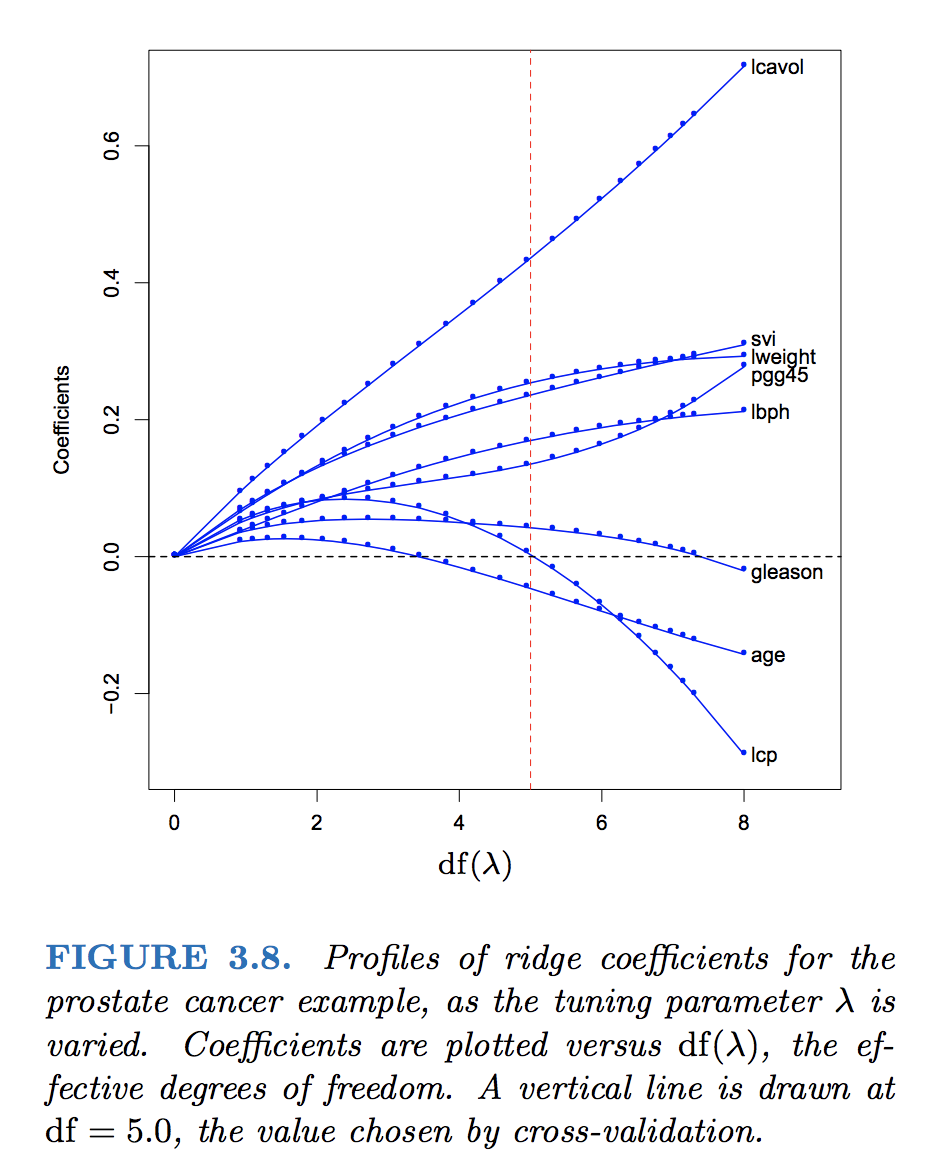
\includegraphics[width=0.84\textwidth, height=0.7\textwidth]{fig_ridge_path.png}
\footnote{%
solution path  of ridge regression, from [ESL]. }
  \end{figure}

\end{frame}

%%%--------------------------------------------------------------------



\frame{

{\color{blue} \huge 
  LASSO }

}

%%%--------------------------------------------------------------------

\frame {

\frametitle{Bridge estimators}

(Frank and Friedman, 1993)

With $L_r(\beta)=\sum_{j=0}^p |\beta_j|^r$,
$$
\hat \beta^{bridge} = \argmin_{\beta} \| {\bf y} - {\bf X} \beta\|^2 + \lambda L_r(\beta)
$$

\begin{itemize}
\item $L_0(\beta) = \sum_{j=0}^p I(\beta_j \neq 0)$; (Hard thresholding)
\item $L_1(\beta) = \sum_{j=0}^p |\beta_j|$; (Lasso)
\item $L_2(\beta) = \sum_{j=0}^p \beta_j^2$; (Ridge regression)
\item $L_{\infty}(\beta) = \max_j~|\beta_j|$.
\end{itemize}

}


%%%--------------------------------------------------------------------

\frame {

\frametitle{ }

\begin{figure}[htb]
\centering
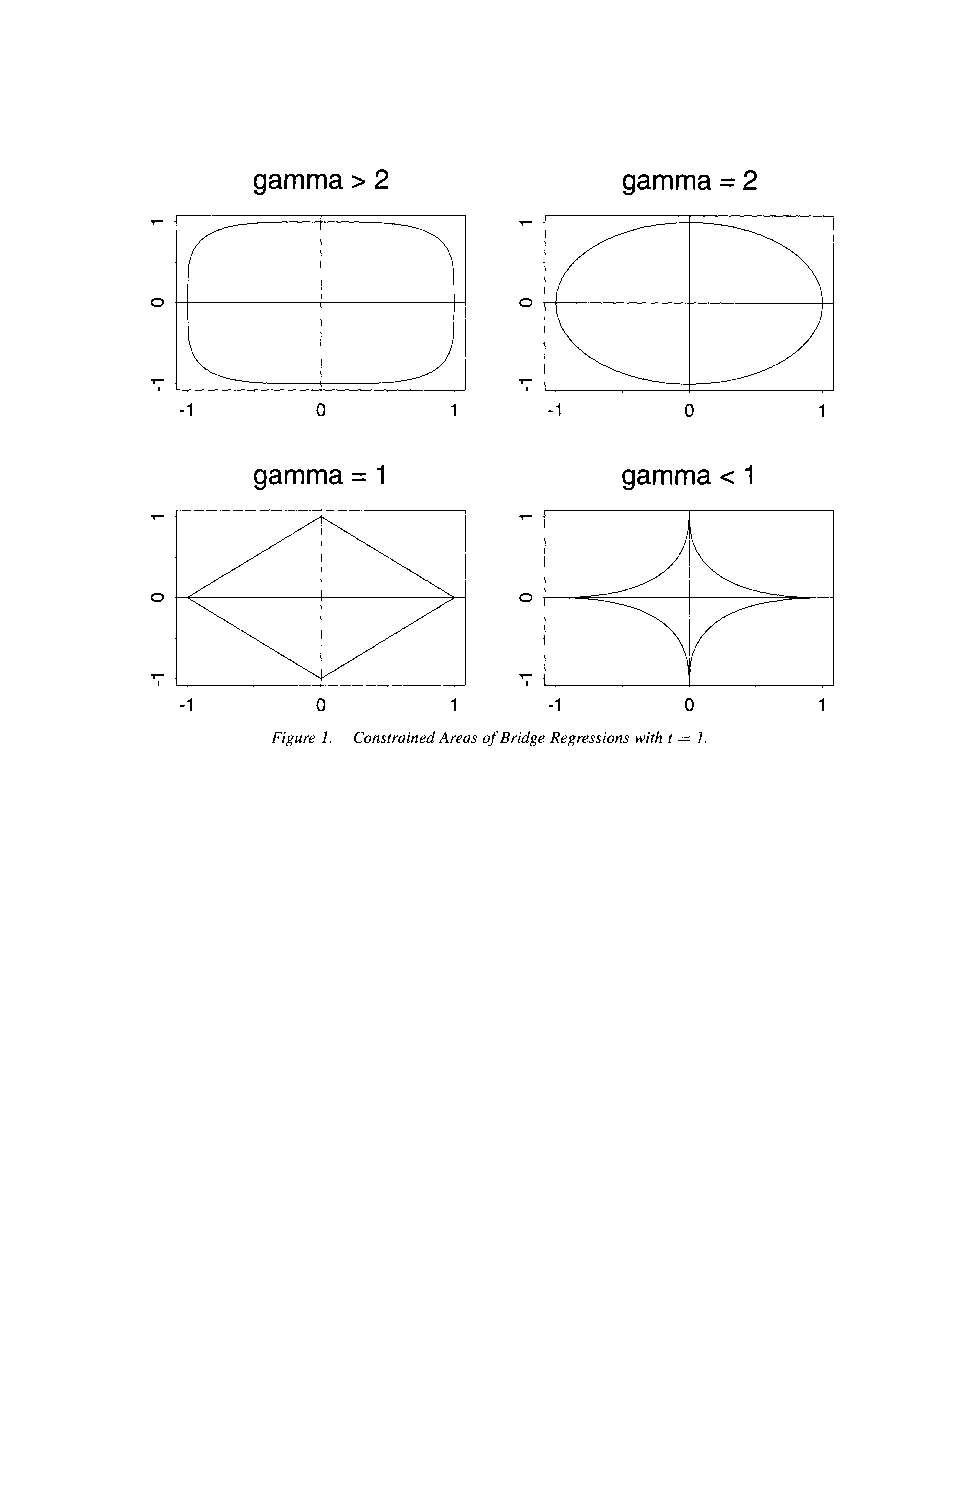
\includegraphics[width=4in]{Chp18_1.pdf}
\end{figure}

}




\begin{frame}{Least Absolute Shrinkage and Selection Operator (Lasso)}
Tibshirani (Journal of the Royal Statistical Society 1996)
introduced the LASSO.
\bigskip
  
  \emph{Lasso estimator}: let $r = 1$ in bridge estimator
  \begin{align*}
    \hat{\beta}^\lambda & = \argmin_\beta
    \left\{ \|{\bf y} - {\bf X} \beta\|_2^2 + \lambda \|\beta\|_1 \right\}, \\
    \hat{\beta}^s
    & = \argmin_{\|\beta\|_1 \le s} \|{\bf y} - {\bf X} \beta\|_2^2,
  \end{align*}
  where $\|\beta\|_1 = \sum_{j=1}^p |\beta_j|$.


  Again  there exists a bijection between $\lambda$ and $s$.


\end{frame}




%%%--------------------------------------------------------------------

\frame {

\frametitle{Sparse solution}

\biz
\item 
Due to the nature of the $l_1$-norm constraint, if $t$ is small enough some coefficients of the lasso solution become {\em exactly} zero.  

\item   The elliptical contour is likely to hit the corner of the polytope,
  corresponding to sparse $\hat{\beta}$. Variable selection: drop the features
  with $\hat{\beta}_j = 0$.

\item  The $l_r$ regularization results in sparsity when $0 \le r \le 1$, and is
  convex when $1 \le r < \infty$. 
  
\item  {\bf Lasso is sparse and convex.}
 Original implementation involves quadratic programming
techniques from convex optimization
\item Efron et al. (Annals of Statistics 2004) proposed {\bf LARS}
({\bf least angle regression}), which computes the LASSO path
efficiently
\biz
\item Interesting modification called is called forward stagewise
\item In many cases it is the same as the LASSO solution
\item Forward stagewise is easy to implement:
\url{http://www-stat.stanford.edu/~hastie/TALKS/nips2005.pdf}
\eiz
\eiz

}



\frame{

\vspace{6mm}
\begin{figure}
\centering
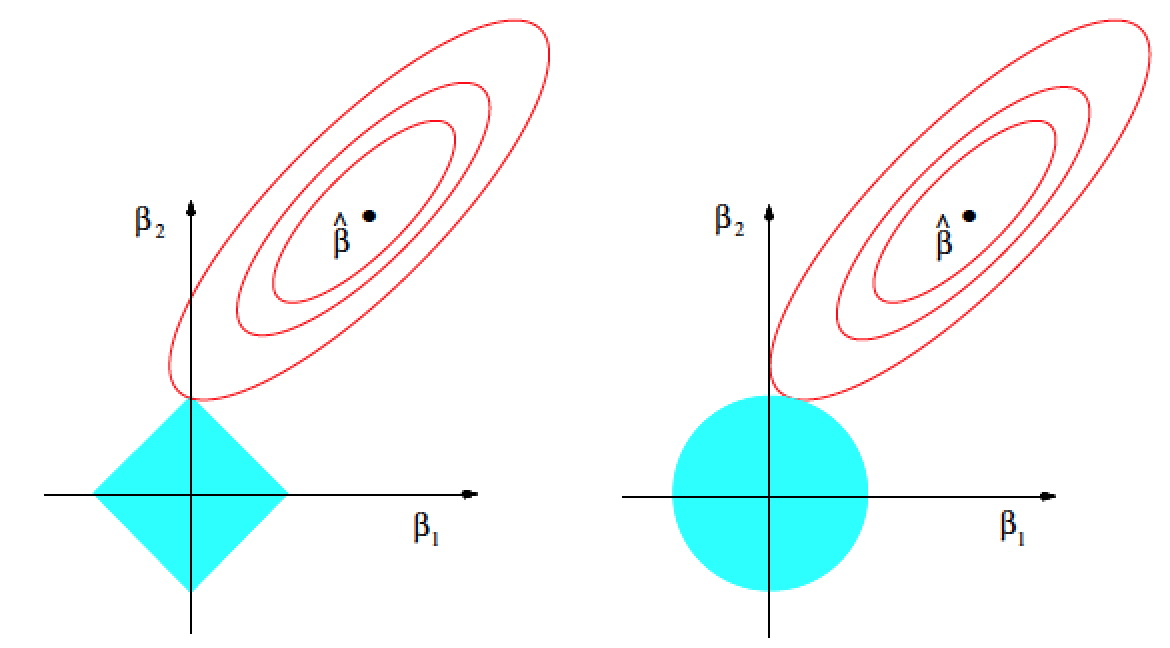
\includegraphics[width=\textwidth]{Figure3_11.png}
\end{figure}
$\bh$ in the center is the $\bh^{OLS}$
}


%%%--------------------------------------------------------------------

\frame {

\frametitle{Ridge vs Lasso}

Consider a simple but illuminating example:
 Show the solutions  
 \begin{align*}
    \hat{\beta}^{ ridge}  & = \argmin_{\beta}
    \left\{ \|  \beta -\bh \|_2^2 + \lambda \|\beta\|^2_2 \right\}, \\
    \hat{\beta}^{ lasso} & = \argmin_{\beta}
    \left\{ \|  \beta -\bh \|_2^2 + \lambda \|\beta\|_1 \right\}  \end{align*}
    are
    
\begin{itemize}
\item $\hat \beta_j^{ridge} = \hat \beta_j / (1+\lambda)$
\item $\hat \beta_j^{lasso} = \sign(\hat \beta_j) (|\hat \beta_j| -\lambda)_+ $  
\end{itemize}
    
 
\href{https://www.desmos.com/calculator/uqt4bgkpky}{visualization
of $\bh^{ridge}$ and $\bh^{lasso}$} from desmos.com webpage

Warning:  taking the traditional derivative for lasso objective function is the wrong way!

Ridge regression shrinks the $\bh$ in all components/directions.
Lasso translates them towards zero by a constant, truncating at zero.
}

\frame{
\begin{figure}
\centering
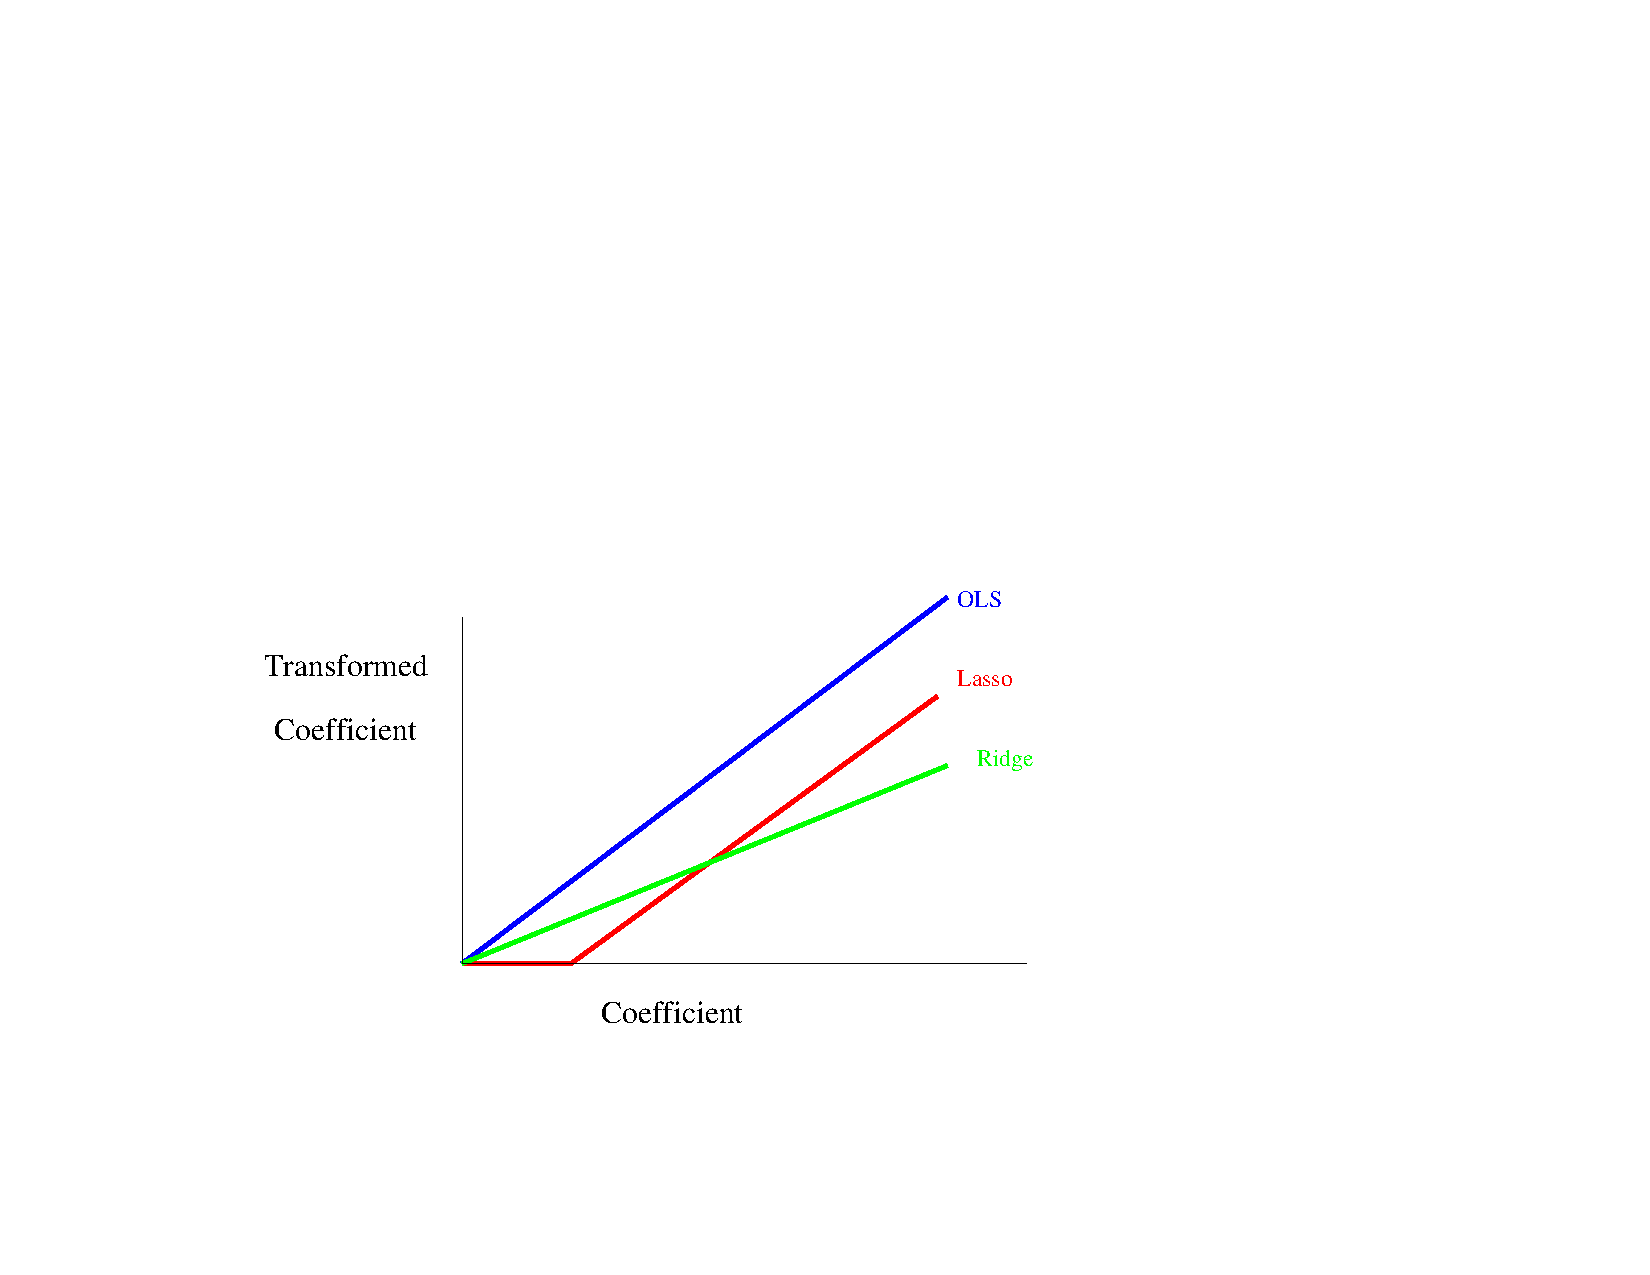
\includegraphics[width=\textwidth]{Chp3_2.pdf}
\end{figure}

}

%%%--------------------------------------------------------------------

\frame {

\frametitle{Solution path}

\begin{itemize}
\item Clearly, the lasso solution $\hat \beta^{lasso}$ changes with the value of $\lambda$
\item Even better, $\hat \beta^{lasso}(\lambda)$ is a \structure{piecewise linear} function of $\lambda$
\item The path algorithm starts at $\lambda=\infty$ or $s=0$, and traces the solution path
by continuously changing $\lambda$ \footnote{homotopy method}. 
Each new $\lambda$-solution is computed successively
by  solving the KKT conditions with a good initial guess set as the 
precise solution for a neighboring old $\lambda$.
\item The key is to find the turning knots $\lambda_1$, \ldots, $\lambda_T$
\item An interesting reading: Efron et al. (AOS; 2003)

\item  Read the reference \href{https://web.stanford.edu/~hastie/Papers/glmnet.pdf}
{Regularization Paths for Generalized Linear Models
via Coordinate Descent}
\item Path algorithms are available for many methods, such as fused lasso, trend filtering, locally adaptive regression splines, SVMs, 1-norm SVMs, relaxed maximum entropy method ...
 \end{itemize}

}


%
%\begin{frame}{Lasso}
%
%  \begin{figure}
%   % \includegraphics[width=0.4\textwidth]{fig_lasso_geo.png}
%    
%    %\includegraphics[width=0.4\textwidth]{fig_lasso_path.png}
%    \caption{%
%      The geometric explanation (left) and regularization path (right) of Lasso.
%      Note that the $x$-axis of the regularization path is the shrinkage factor
%      $s = t / \sum_{j=1}^d |\hat{\beta}_j|$.
%    }\footnote{%
%      Trevor Hastie et al. (2008). The Elements of Statistical Learning: Data
%      Mining, Inference, and Prediction. Figure 3.11 and 3.8.
%    }
%  \end{figure}
%
%\end{frame}


%%%--------------------------------------------------------------------
\frame{


The motivation for the Lasso came from an interesting proposal of Breiman
(1993). Breiman's non-negative Garotte minimizes

$$
\min_{ c_j \geq 0, \forall j}~\frac{1}{2} \sum_{i=1}^n \big (y_i - \sum_{j=1}^p c_j \hat \beta_j x_{ij} \big )^2 + \lambda \sum_{j=1}^p c_j
$$
and then $\hat \beta_j^{ng} = \hat c_j \hat \beta_j$.
\begin{ex}
Show when $\X^\tr\X = n \eye$,  the non-negative Garotte  estimator
is
$$
\hat \beta_j^{ng} = \left ( 1-\frac{\lambda}{2 \hat \beta_j^2} \right )_+ \hat \beta_j.
$$
\end{ex}


 \begin{itemize}
\item It shrinks small $|\hat \beta_j|$ to zero.
  It is almost unbiased for large $|\hat \beta_j|$.
\item   Garotte starts with the OLS estimates and shrinks them by non-negative
factors whose sum is constrained.
\item  In
contrast,   Lasso avoids the explicit use of the OLS estimates.
\item Lasso is also closely related to the wavelet soft-thresholding method by Donoho
and Johnstone (1994),   and boosting method.
\end{itemize}
}


%%%%%-----------
\frame {

 
One can just focus on the component-wise formulation
$$
\min_{\beta}~\frac{1}{2} (z_j - \beta_j)^2 + J(|\beta_j|)
$$

\begin{itemize}
\item Hard thresholding: $J(|\beta_j|) = \lambda^2 - (|\beta_j|-\lambda)^2 I(|\beta_j|<\lambda)$, then\footnote{the proof is exercise }
    $$
    \hat \beta_j = z_j I(|z_j| > \lambda).
    $$
\item Soft thresholding (Lasso): $J(|\beta_j|) = \lambda |\beta_j|$, then
    $$
    \hat \beta_j = \sign(z_j) (|z_j|-\lambda)_+.
    $$
\end{itemize}

}



%%%--------------------------------------------------------------------



%%%--------------------------------------------------------------------

\frame {

\frametitle{SCAD (Fan and Li, 2001; JASA)}

$$
\min_{\beta}~\frac{1}{2} \| {\bf y} - {\bf X} \beta\|^2 + \sum_{j=1}^p q_{\lambda}(|\beta_j|),
$$
where
$$
q_{\lambda}(\beta) = \left \{
\begin{array}{ll}
\lambda \beta & \mbox{if}~|\beta| \leq \lambda, \\
-\frac{(|\beta|^2-2a\lambda |\beta|+\lambda^2)}{2(a-1)} & \mbox{if}~\lambda < |\beta| \leq a \lambda, \\
\frac{(a+1)\lambda}{2} & \mbox{if}~|\beta| > a \lambda.
\end{array}
\right .
$$

\begin{itemize}
\item Similar to the truncated lasso penalty, but it is smooth everywhere.
\end{itemize}
}



%%%--------------------------------------------------------------------

\frame {

\frametitle{ }

\begin{figure}[htb]
\centering
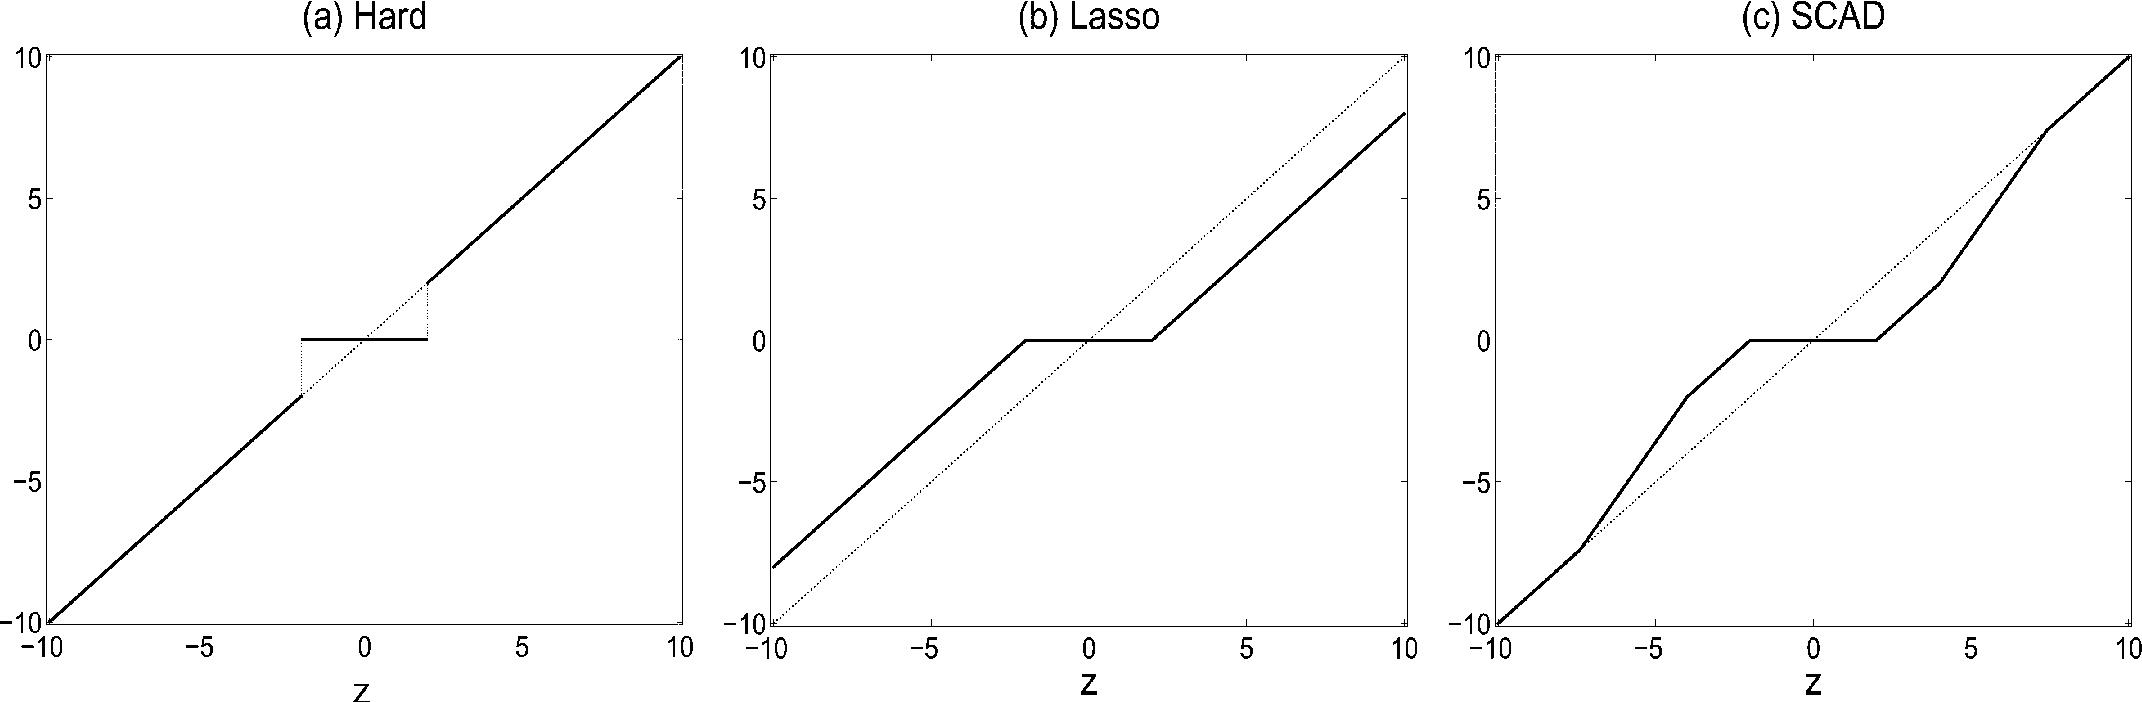
\includegraphics[width=\textwidth]{Chp18_2.png}
\end{figure}
Reference:
 Antoniadis and Fan (2001);  Fan and Li (2001)
}

\frame{
{Revisit Bias-Variance (again !)}
\biz
\item
In the beginning,
We calculated the MSE for ordinary least square
where the bias vanishes.
\item We  now focus on
the ridge regression, 
$\bh^{\lambda}=(\XX+\lambda \eye)^{-1}\X \y$, where $\lambda>0$ is the 
penalty parameter.
The corresponding MSE for $\bh^{\lambda}$
at the new testing point $x_0$ then is written as
\footnote{again, the training data's $\X$  part is fixed or conditioned.}
\begin{align*}
\MSE^{\lambda} (x_0)
=&\var_{\y}(x_0^\tr \bh^{\lambda})
+ \left( \e_\y   (x_0^\tr \bh^{\lambda}) -f(x_0)  \right)^2
\\
=&\var_{\y}(x^\tr_0 (\XX+\lambda \eye)^{-1}\X^\tr \y)
+ \left(    x_0^\tr \e_\y( \bh^{\lambda}) -f(x_0)  \right)^2
\\
=& \sigma^2_\eps   \norm{ {\bf h}_\lambda x_0 }_2^2
+ \left(    x_0^\tr  (\XX+\lambda \eye)^{-1}  \X^\tr \X\beta  - x_0^\tr \beta  \right)^2
\end{align*}
\eiz
where ${\bf h}_\lambda=\X (\XX+\lambda \eye)^{-1} $.
Exercise: with the aid of SVD, find the minimum point 
$\lambda$ for $\MSE^\lambda$.
}


\frame{{Decomposition of  average squared bias}
\biz
\item
Note that   we have \underline{assumed} that 
{the ground truth 
is a linear model $f(x)=x^\tr\beta$.}
\item
From now we do not assume $f$ is linear 
and it could be a nonlinear function for a general consideration. 
This is a more realistic setting.
\item
The additive error model  $Y=f(X)+\eps$  is  still assumed for data.
\item The best-fitting approximation
 in the {\it linear model class} \footnote{In other words, $x\to x^\tr \beta^*$ is  $f_\Hcal(x)$ defined in Topic  1 ($\Hcal$ is hypothesis space)} 
 is  given by 
 $$\beta^* =\argmin_{\beta} \e_{X} (f(X)- X^\tr \beta)^2
$$
\item Note that  $\beta_*$ satisfies the normal equation:
$$  \e(X^\tr X)\beta_* = \e[ f(X)X] $$
\eiz
}

\frame{
{Decomposition of average (squared) bias}
\biz
\item We still consider the $\MSE^{\lambda}$ for the ridge 
regression. The variance part $\var(x_0^\tr \bh^{\lambda})$ is unchanged.
Now  the squared  bias becomes
{\footnotesize
$
\left(    x_0^\tr \e_\y( \bh^{\lambda}) -f(x_0)  \right)^2
=
\left(    x_0^\tr \e_\y( \bh^{\lambda}) -x_0^\tr \beta_*
+x_0^\tr \beta_* -f(x_0)  \right)^2
=\left(    x_0^\tr \e_\y( \bh^{\lambda}) -x_0^\tr \beta_*\right)^2
+ \left(x_0^\tr \beta_* -f(x_0)  \right)^2
+2 \left(    x_0^\tr \e_\y( \bh^{\lambda}) -x_0^\tr \beta_*\right)
 \left(x_0^\tr \beta_* -f(x_0) \right)
$}
\item 
Taking expectation for $x_0\sim X$ and using the normal equation, we have the average squared bias is 
\begin{align*}
&\e_{x_0}\left(    x_0^\tr \e_\y( \bh^{\lambda}) -f(x_0)  \right)^2
\\
=&
\underbrace
{
\e_{x_0}  \left(    x_0^\tr  ( \e_\y  \bh^{\lambda} -  \beta_*)\right)^2
}
_{
\text{Ave (Estimation Bias}^2) 
}
+ \underbrace
{
\e_{x_0}  \left(x_0^\tr \beta_* -f(x_0)  \right)^2
}
_{
\text{Ave (Model Bias}^2)
}
\end{align*}
This is equation (7.14) in [ELS].
\eiz
}

%%%%%-------------
\frame
{ {Remarks}
\biz 
\item Model Bias, by definition, 
involves the ground truth, which is not accessible;  Estimation Bias, by definition,
involves $\beta^*$, which is not accessible either.
\item However, this decomposition is conceptually 
inspiriting  to  have Model Bias.
\item The Model Bias corresponds to the approximation error 
in Topic 1  ($f_\Hcal$ vs $f^*$)
and the Estimation Bias is similar to  the sampling error in Topic 1
($\hat{f}_\Dcal$ vs $f_\Hcal$).
In approximation theory viewpoint, the variance $\var_{\Dcal}
\hat{f}_\Dcal$ is not considered.

\item Ridge method and LASSO further restricts the linear model 
$\Hcal_{linear}$
to a smaller set
in the form  $\Hcal_\lambda:=\set{f: f(x)=\beta^\tr x ,  \|\beta\|\leq \lambda}$; 
they affect the estimation bias (and the variance of the prediction). 
The improvement of Model Bias 
 needs go from linear to nonlinear 
 if the ground truth is far away from being linear.

\eiz
}


%%%--------------------------------------------------------------------
%
%
%\begin{frame}{The Persistency Theory of Lasso}
%
%  \textit{Proof.} First, we have showed that
%  \[
%    L(\hat{\beta}) - \inf_{\|\beta\|_1 \le C} L(\beta)
%    \le 2 \sup_{\|\beta\|_1 \le C} |\hat{L}_n (\beta) - L(\beta)|.
%  \]
%
%  Let $Z = {(Y, X^\intercal)}^\intercal$, $z_i = {(y_i,
%  x_i^\intercal)}^\intercal$ and $\gamma = {(-1, \beta^\intercal)}^\intercal$,
%  then
%  \[
%    L(\beta)
%    = \mathbb{E}[\gamma^\intercal Z Z^\intercal \gamma]
%    = \gamma^\intercal \Sigma \gamma, \quad
%    \hat{L}_n (\beta)
%    = \frac{1}{n} \sum_{i=1}^n \gamma^\intercal z_i z_i^\intercal \gamma
%    = \gamma^\intercal \hat{\Sigma} \gamma,
%  \]
%  where $\Sigma = \mathbb{E} [Z Z^\intercal]$ and $\hat{\Sigma} = \frac{1}{n}
%  \sum_{i=1}^n z_i z_i^\intercal$. We have
%  \[
%    |\hat{L}_n (\beta) - L(\beta)|
%    = |\gamma^\intercal (\hat{\Sigma} - \Sigma) \gamma|
%    \le \|\gamma\|_1 \|(\hat{\Sigma} - \Sigma) \gamma\|_\infty
%    \le \|\gamma\|_1^2 \max_{j, k} |\hat{\Sigma}_{jk} - \Sigma_{jk}|,
%  \]
%  thus
%  \[
%    \sup_{\|\beta\|_1 \le C} |\hat{L}_n (\beta) - L(\beta)|
%    \le {(1 + C)}^2 \max_{j, k} |\hat{\Sigma}_{jk} - \Sigma_{jk}|.
%  \]
%
%\end{frame}

%
%
%
%\begin{frame}{The Persistency Theory of Lasso}
%
%  \begin{defn}[Persistence]
%    Let $L(f)$ be the prediction error of function $f$.  An estimator $\hat{f}$
%    is persistent within a class $\mathcal{F}$ if
%    \[
%      L(\hat{f}) - \inf_{f \in \mathcal{F}} L(\beta)
%      \stackrel{P}{\longrightarrow} 0 \quad \text{as } n \to \infty.
%    \]
%  \end{defn}
%
%  \begin{thm}[Persistence of Lasso]
%    Assume that the random variables $\|X\|_\infty \le B$ and $|Y| \le B$. Let
%    $L(\beta) = \mathbb{E} |Y - \beta^\intercal X|^2$ and $\hat{L}_n =
%    \frac{1}{n} \sum_{i=1}^n |y_i - \beta^\intercal x_i|^2$ where $(x_i, y_i)$
%    are random samples. The Lasso estimator $\hat{\beta} = \argmin_{\|\beta\|_1
%    \le C} \hat{L}_n (\beta)$. Then with probability $1 - \Delta$,
%    \[
%      L(\hat{\beta}) - \inf_{\|\beta\|_1 \le C} L(\beta)
%      \le 2 {(1 + C)}^2
%      \sqrt{\frac{2 B^4}{n} \log\left(\frac{2 d^2}{\Delta} \right)}.
%    \]
%  \end{thm}
%
%\end{frame}
%

%
%
%
%\begin{frame}{The Persistency Theory of Lasso}
%
%  \begin{lem}[Hoeffding]
%    Let random variables $X_1, {\bf D}ots, X_n$ i.i.d.\@ with $|X_i| \le C$, then
%    \[
%      \mathbb{P}\left\{
%        \left|\frac{1}{n}\sum_{i=1}^n X_i - \mathbb{E} X_i \right| > t
%      \right\} \le 2 e^{-\frac{n t^2}{2 C^2}}.
%    \]
%  \end{lem}
%
%  Since $\|Z\|_\infty \le B$, we have
%  \[
%    \mathbb{P}\left\{ \max_{j, k} |\hat{\Sigma}_{jk} - \Sigma_{jk}| > t \right\}
%    \le d^2 \mathbb{P}\{|\hat{\Sigma}_{jk} - \Sigma_{jk} > t\}
%    \le 2 d^2 e^{-\frac{n t^2}{2 B^4}}.
%  \]
%  Setting $\Delta = 2 d^2 e^{-\frac{n t^2}{2 B^4}}$, we have $t = \sqrt{\frac{2
%  B^4}{n} \log\left(\frac{2 d^2}{\Delta} \right)} $, which finishes the proof.
%
%\end{frame}
%

\end{document}

